%-*- coding: UTF-8 -*-
% 论文总结.tex
% 2020年7月第一周
\documentclass[UTF8]{ctexart}
\usepackage{graphicx}
\usepackage{float}
\usepackage{amsmath}
\usepackage{geometry}
\geometry{a4paper,centering,scale=0.8}
\usepackage[format=hang,font=small,textfont=it]{caption}
\usepackage[nottoc]{tocbibind}
\usepackage{url}
\usepackage{listings}
\usepackage{booktabs}
\usepackage{xcolor}     %高亮使用的颜色
\definecolor{commentcolor}{RGB}{85,139,78}
\definecolor{stringcolor}{RGB}{206,145,108}
\definecolor{keywordcolor}{RGB}{34,34,250}
\definecolor{backcolor}{RGB}{220,220,220}

\lstset{
 columns=fixed,       
 numbers=left,                                        % 在左侧显示行号
 numberstyle=\tiny\color{gray},                       % 设定行号格式
 frame=none,                                          % 不显示背景边框
 backgroundcolor=\color[RGB]{245,245,244},            % 设定背景颜色
 keywordstyle=\color[RGB]{40,40,255},                 % 设定关键字颜色
 numberstyle=\footnotesize\color{darkgray},           
 commentstyle=\it\color[RGB]{0,96,96},                % 设置代码注释的格式
 stringstyle=\rmfamily\slshape\color[RGB]{128,0,0},   % 设置字符串格式
 showstringspaces=false,                              % 不显示字符串中的空格
 language=c++,                                        % 设置语言
}

\newenvironment{myquote}
{\begin{quote}\kaishu\zihao{-5}}
{\end{quote}}

\newcommand\degree{^\circ}

\title{\heiti Real_Time Multistep Attack Prediction Based on Hidden Markov Models}
\author{\kaishu 海华}
\date{\today}

\bibliographystyle{plain}

\newtheorem{thm}{定理}

\begin{document}
    \maketitle

    \clearpage

    \section{总结}\label{sec:diyijie}
  	本论文提出了一种基于隐马尔可夫模型的方法来利用IDS警报预测多步攻击。IDS日志将告警处理为observes定义了tag和severity,其中tag是CVE报告中定义的漏洞描述提取词,severity为日志中告警等级字段。

	框架设计包含部分:多步攻击文件(Multistep Attack files,pcap格式,用于HMM模型训练阶段),离线训练阶段,HMM配置文件(离线训练生成的参数,参数涵盖了状态转移可能性矩阵和马尔科夫状态链中状态的数目,主要用于预测阶段),预测模型利用HMM配置文件对IDS日志中的告警序列进行预测,计算攻击的可能性。

	隐马尔可夫模型抽象成一个 ,第一个参数表示基于IDS告警和CVE报告的观察序列。第二个参数表示攻击状态。第三个参数表示状态转换可能性矩阵。第四个参数表示 an observation probability matrix,其实就是observation到S的可能性矩阵。第五个参数表示初始状态可能性向量。增加H向量表示每一步攻击状态的平均告警数。增加H后表示的六元祖向量可用于计算最后的攻击可能性。训练阶段分别采用监督学习方式和无监督学习方式。 其中可以学习一下Baum-Welch算法是最常用的算法。还有其他的最大似然估计、梯度下降算法等。最后通过构建的六元祖结合训练的配置文件参数计算状态可能性和攻击可能性。最后论文的第7部分讲解了具体算法的实现实例,第八部分讲解了不同攻击场景构建的攻击配置文件。
	\begin{figure}[ht]
        \centering
        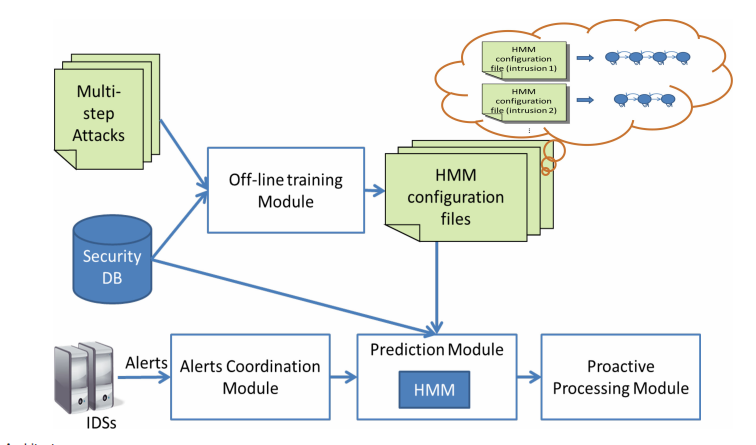
\includegraphics[scale=0.5]{picture/001.png}
        \caption{框架}
        \label{fig:001}
    \end{figure}

	本文创新:
	\begin{itemize}
	\item[1] 构建的六元祖模型,在原隐马尔可夫模型的基础上引入了状态的平均告警数目。
	\item[2] observation 状态基于CVE报告和日志告警等级。
	\item[3] 本文的实验对性能、状态和攻击可能性、分布式攻击场景中算法的应用进行了分析。
	\end{itemize}
	\clearpage
	
	\bibliography{test}
\end{document}

